\section{Overview}

The software to be is designed as a Client-Server system with a three-tier architecture: Presentation Level, Business Logic or Application Layer and Data Access Layer. In particular:
\begin{itemize}
	\item \textbf{Presentation Level}: handles the interaction with Customers and Store Managers. It contains the interfaces able to communicate with them and it is responsible for rendering of the information. Its scope is to make understandable the functions of the application to the users. In particular, this levels provides an interface both to the Customer (a mobile application) and Store Manager (a web application) in order to allow them to exploit, in a simple way, all the services of the application. The purpose is to make them as efficient and intuitive as possible.

	\item \textbf{Business logic or Application layer}: takes care of the functions to be provided for the users. It also coordinates the work of the application, making logical decisions and moving data between the other two layers. In particular, it contains the Web Server and the Application Server.

	\item \textbf{Data Access Layer}: cares for the management of the information, with the corresponding access to the databases. It picks up useful informations in the database and passes them along the other layers.
\end{itemize}

This architecture has been chosen in order to make the software scalable and flexible to future integrations and modifications, without giving up a fair robustness and a good user experience. The communication between the various components is managed through the exchange of requests and responds, so, some of the main design choices have been taken in order to optimize the expenditure of the available resources. The client software is of limited complexity, acting in many cases only as an interface to the servers and computing only the essential functionalities. The Application Server is used to manage the main application logic; moreover, it contains the management of some of the functions that users do not need to access, or the ones that require an high expenditure of resources. One of the main purposes of the Application Server is to send requests to the database (in the Data Access Layer); in particular, by communicating with its DBMS it can handle, when necessary, all the operations of reading, writing and uploading of data.

\begin{figure}[H]
\centerline{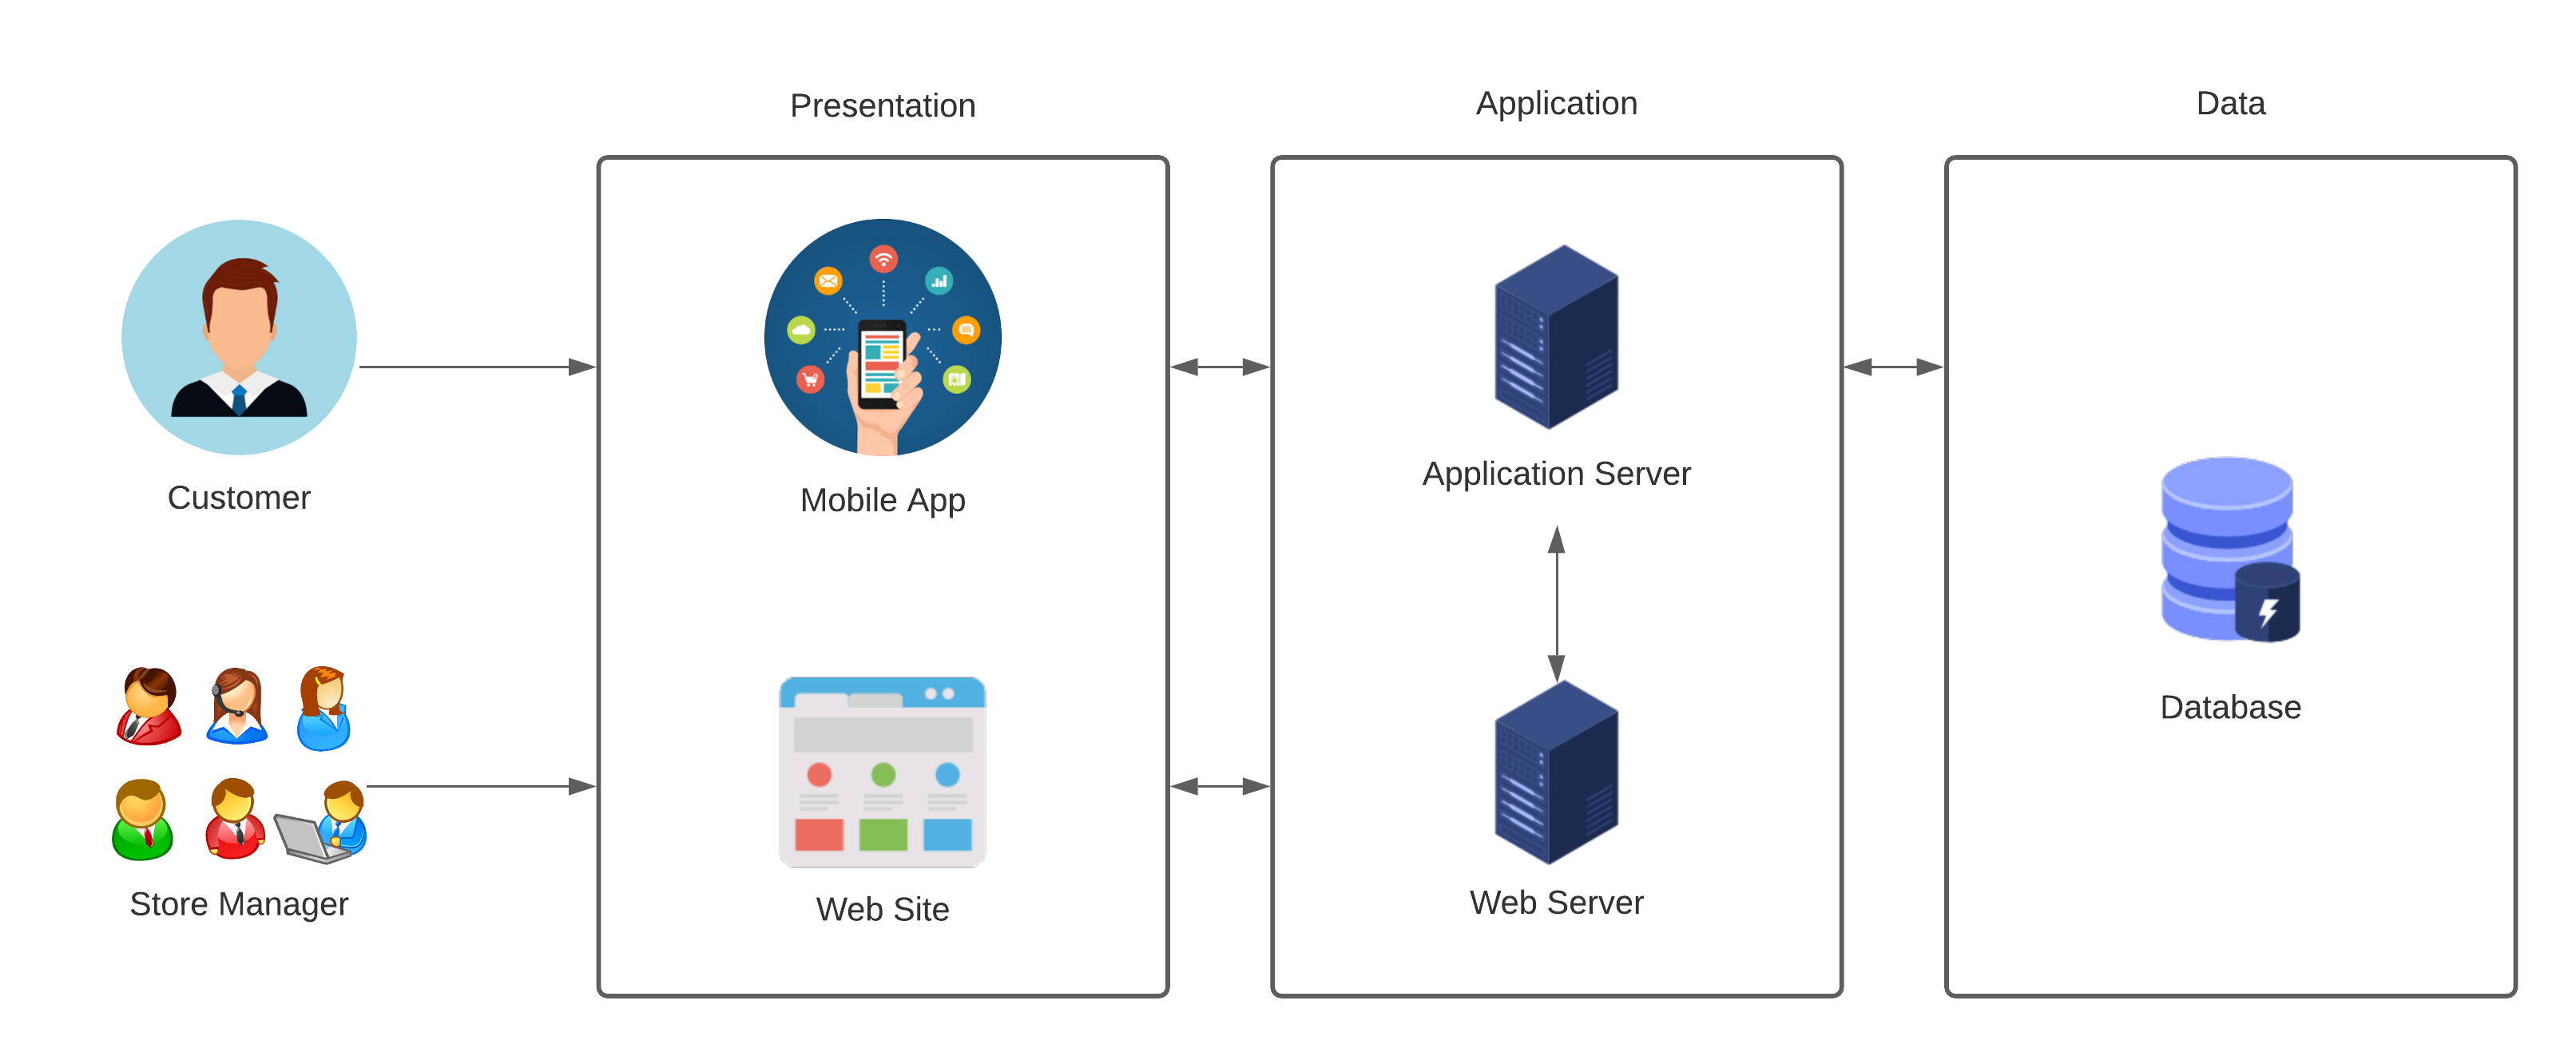
\includegraphics[scale=0.65]{./High-Level}}
\caption{High-Level View of the Application Architecture}
\end{figure}

\subsection{Class Diagram}
The following Class Diagram shows the main entities of the problem, from the requirements point of view.
A more detailed and implementation-oriented Class Diagram will be provided in the Design Document.
\begin{figure}[H] 
\centerline{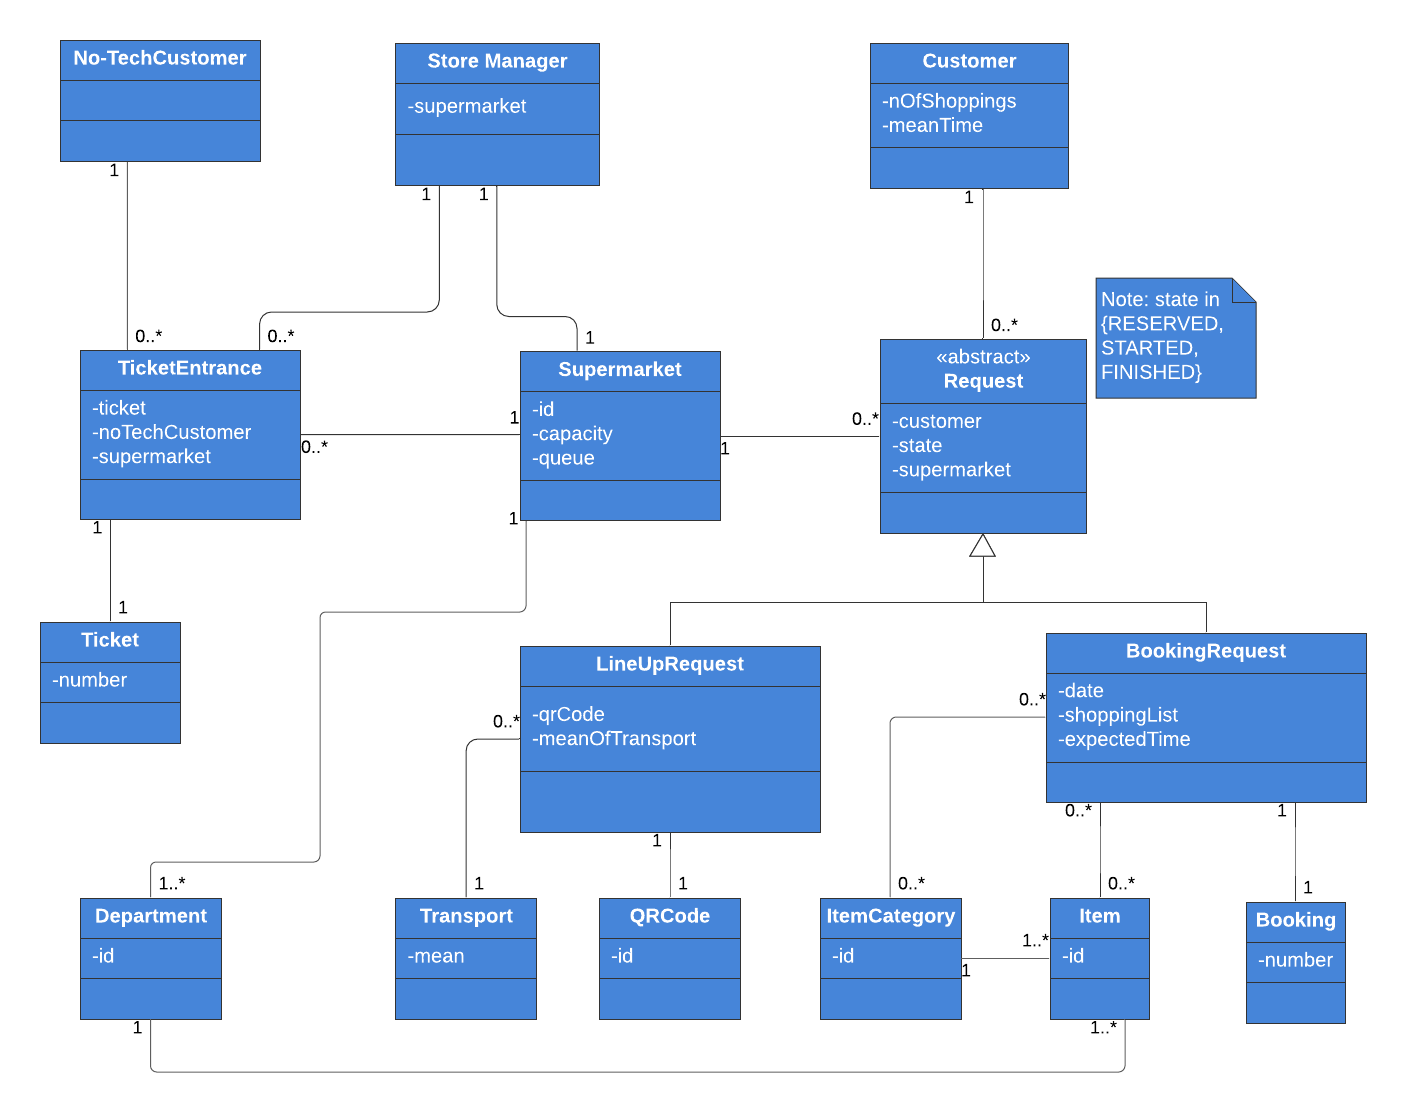
\includegraphics[scale=0.75]{ClassDiagramRASD}}
\caption{Class Diagram}
\end{figure}




 
 

